% Options for packages loaded elsewhere
\PassOptionsToPackage{unicode}{hyperref}
\PassOptionsToPackage{hyphens}{url}
%
\documentclass[
]{article}
\usepackage{amsmath,amssymb}
\usepackage{lmodern}
\usepackage{iftex}
\ifPDFTeX
  \usepackage[T1]{fontenc}
  \usepackage[utf8]{inputenc}
  \usepackage{textcomp} % provide euro and other symbols
\else % if luatex or xetex
  \usepackage{unicode-math}
  \defaultfontfeatures{Scale=MatchLowercase}
  \defaultfontfeatures[\rmfamily]{Ligatures=TeX,Scale=1}
\fi
% Use upquote if available, for straight quotes in verbatim environments
\IfFileExists{upquote.sty}{\usepackage{upquote}}{}
\IfFileExists{microtype.sty}{% use microtype if available
  \usepackage[]{microtype}
  \UseMicrotypeSet[protrusion]{basicmath} % disable protrusion for tt fonts
}{}
\makeatletter
\@ifundefined{KOMAClassName}{% if non-KOMA class
  \IfFileExists{parskip.sty}{%
    \usepackage{parskip}
  }{% else
    \setlength{\parindent}{0pt}
    \setlength{\parskip}{6pt plus 2pt minus 1pt}}
}{% if KOMA class
  \KOMAoptions{parskip=half}}
\makeatother
\usepackage{xcolor}
\usepackage[margin=1in]{geometry}
\usepackage{color}
\usepackage{fancyvrb}
\newcommand{\VerbBar}{|}
\newcommand{\VERB}{\Verb[commandchars=\\\{\}]}
\DefineVerbatimEnvironment{Highlighting}{Verbatim}{commandchars=\\\{\}}
% Add ',fontsize=\small' for more characters per line
\usepackage{framed}
\definecolor{shadecolor}{RGB}{248,248,248}
\newenvironment{Shaded}{\begin{snugshade}}{\end{snugshade}}
\newcommand{\AlertTok}[1]{\textcolor[rgb]{0.94,0.16,0.16}{#1}}
\newcommand{\AnnotationTok}[1]{\textcolor[rgb]{0.56,0.35,0.01}{\textbf{\textit{#1}}}}
\newcommand{\AttributeTok}[1]{\textcolor[rgb]{0.77,0.63,0.00}{#1}}
\newcommand{\BaseNTok}[1]{\textcolor[rgb]{0.00,0.00,0.81}{#1}}
\newcommand{\BuiltInTok}[1]{#1}
\newcommand{\CharTok}[1]{\textcolor[rgb]{0.31,0.60,0.02}{#1}}
\newcommand{\CommentTok}[1]{\textcolor[rgb]{0.56,0.35,0.01}{\textit{#1}}}
\newcommand{\CommentVarTok}[1]{\textcolor[rgb]{0.56,0.35,0.01}{\textbf{\textit{#1}}}}
\newcommand{\ConstantTok}[1]{\textcolor[rgb]{0.00,0.00,0.00}{#1}}
\newcommand{\ControlFlowTok}[1]{\textcolor[rgb]{0.13,0.29,0.53}{\textbf{#1}}}
\newcommand{\DataTypeTok}[1]{\textcolor[rgb]{0.13,0.29,0.53}{#1}}
\newcommand{\DecValTok}[1]{\textcolor[rgb]{0.00,0.00,0.81}{#1}}
\newcommand{\DocumentationTok}[1]{\textcolor[rgb]{0.56,0.35,0.01}{\textbf{\textit{#1}}}}
\newcommand{\ErrorTok}[1]{\textcolor[rgb]{0.64,0.00,0.00}{\textbf{#1}}}
\newcommand{\ExtensionTok}[1]{#1}
\newcommand{\FloatTok}[1]{\textcolor[rgb]{0.00,0.00,0.81}{#1}}
\newcommand{\FunctionTok}[1]{\textcolor[rgb]{0.00,0.00,0.00}{#1}}
\newcommand{\ImportTok}[1]{#1}
\newcommand{\InformationTok}[1]{\textcolor[rgb]{0.56,0.35,0.01}{\textbf{\textit{#1}}}}
\newcommand{\KeywordTok}[1]{\textcolor[rgb]{0.13,0.29,0.53}{\textbf{#1}}}
\newcommand{\NormalTok}[1]{#1}
\newcommand{\OperatorTok}[1]{\textcolor[rgb]{0.81,0.36,0.00}{\textbf{#1}}}
\newcommand{\OtherTok}[1]{\textcolor[rgb]{0.56,0.35,0.01}{#1}}
\newcommand{\PreprocessorTok}[1]{\textcolor[rgb]{0.56,0.35,0.01}{\textit{#1}}}
\newcommand{\RegionMarkerTok}[1]{#1}
\newcommand{\SpecialCharTok}[1]{\textcolor[rgb]{0.00,0.00,0.00}{#1}}
\newcommand{\SpecialStringTok}[1]{\textcolor[rgb]{0.31,0.60,0.02}{#1}}
\newcommand{\StringTok}[1]{\textcolor[rgb]{0.31,0.60,0.02}{#1}}
\newcommand{\VariableTok}[1]{\textcolor[rgb]{0.00,0.00,0.00}{#1}}
\newcommand{\VerbatimStringTok}[1]{\textcolor[rgb]{0.31,0.60,0.02}{#1}}
\newcommand{\WarningTok}[1]{\textcolor[rgb]{0.56,0.35,0.01}{\textbf{\textit{#1}}}}
\usepackage{graphicx}
\makeatletter
\def\maxwidth{\ifdim\Gin@nat@width>\linewidth\linewidth\else\Gin@nat@width\fi}
\def\maxheight{\ifdim\Gin@nat@height>\textheight\textheight\else\Gin@nat@height\fi}
\makeatother
% Scale images if necessary, so that they will not overflow the page
% margins by default, and it is still possible to overwrite the defaults
% using explicit options in \includegraphics[width, height, ...]{}
\setkeys{Gin}{width=\maxwidth,height=\maxheight,keepaspectratio}
% Set default figure placement to htbp
\makeatletter
\def\fps@figure{htbp}
\makeatother
\setlength{\emergencystretch}{3em} % prevent overfull lines
\providecommand{\tightlist}{%
  \setlength{\itemsep}{0pt}\setlength{\parskip}{0pt}}
\setcounter{secnumdepth}{-\maxdimen} % remove section numbering
\usepackage{booktabs}
\usepackage{longtable}
\usepackage{array}
\usepackage{multirow}
\usepackage{wrapfig}
\usepackage{float}
\usepackage{colortbl}
\usepackage{pdflscape}
\usepackage{tabu}
\usepackage{threeparttable}
\usepackage{threeparttablex}
\usepackage[normalem]{ulem}
\usepackage{makecell}
\usepackage{xcolor}
\ifLuaTeX
  \usepackage{selnolig}  % disable illegal ligatures
\fi
\IfFileExists{bookmark.sty}{\usepackage{bookmark}}{\usepackage{hyperref}}
\IfFileExists{xurl.sty}{\usepackage{xurl}}{} % add URL line breaks if available
\urlstyle{same} % disable monospaced font for URLs
\hypersetup{
  pdftitle={P8108 Homework 3},
  pdfauthor={Ryan Wei, rw2844},
  hidelinks,
  pdfcreator={LaTeX via pandoc}}

\title{P8108 Homework 3}
\author{Ryan Wei, rw2844}
\date{2022-09-28}

\begin{document}
\maketitle

\hypertarget{problem-1}{%
\subsection{Problem 1}\label{problem-1}}

\begin{table}[!h]

\caption{\label{tab:hand-draw-lifetable}Life table estimate}
\centering
\begin{tabular}[t]{rlrrrrrrrr}
\toprule
Interval & Time Period & $d_i$ & $c_i$ & $n_i$ & $n_i^{\prime}$ & $S(t)$ & $f(t)$ & $h(t)$ & $se(S(t))$\\
\midrule
1 & {}[0,4) & 2 & 1 & 20 & 19.5 & 1.0000 & 0.0257 & 0.2703 & 0.0000\\
2 & {}[4,8) & 1 & 1 & 17 & 16.5 & 0.8974 & 0.0136 & 0.0156 & 0.0687\\
3 & {}[8,12) & 0 & 3 & 15 & 13.5 & 0.8430 & 0.0000 & 0.0000 & 0.0833\\
4 & {}[12,16) & 1 & 2 & 12 & 11.0 & 0.8430 & 0.0192 & 0.0238 & 0.0833\\
5 & {}[16,20) & 1 & 3 & 9 & 7.5 & 0.7664 & 0.0256 & 0.0357 & 0.1053\\
\addlinespace
6 & {}[20,24) & 1 & 1 & 5 & 4.5 & 0.6642 & 0.0369 & 0.0625 & 0.1318\\
7 & {}[24,$\infty$) & 0 & 3 & 3 & 1.5 & 0.5166 & NA & NA & 0.1657\\
\bottomrule
\multicolumn{10}{l}{\rule{0pt}{1em}\textit{Note: } Survival functions estimated at the begining of each interval}\\
\end{tabular}
\end{table}
\newpage

\hypertarget{problem-2}{%
\subsection{Problem 2}\label{problem-2}}

\textbf{Proof}

Since

\[
\begin{aligned}
\hat h(t_{mi}) & = \frac{d_i}{[(t_i -t_{i-1})(\frac{n_i^{\prime} - d_i}{2})]}\\
\hat f(t_{mi}) & = \frac{\hat S_L(t_{i-1})- \hat S_L(t_{i})}{t_i - t_{i-1}}\\
\hat S(t_{mi}) & = \frac{\hat S_L(t_{i-1}) + \hat S_L(t_{i})}{2}\\
\hat S_L(t_i) & = \hat S_L(t_{i-1})(1- \frac{d_i}{n_i^{\prime}})
\end{aligned}
\] Therefore, based on the definition, \[
\begin{aligned}
\hat h(t_{mi}) & = \frac{\hat f(t_{mi})}{\hat S(t_{mi})}\\
& = \frac{2\hat f(t_{mi})}{\hat S_L(t_{i-1}) + \hat S_L(t_{i})}\\
& = \frac{2(\hat S_L(t_{i-1}) - \hat S_L(t_{i}))}{(t_i - t_{i-1})(\hat S_L(t_{i-1}) + \hat S_L(t_{i}))}\\
& = \frac{2(\hat S_L(t_{i-1})\times\frac{d_i}{n_i^{\prime}})}{(t_i - t_{i-1})(\hat S_L(t_{i-1})\times\frac{2n_i^{\prime}-d_i}{n_i^{\prime}})}\\
& = \frac{d_i}{(n_i^{\prime}-\frac{d_i}{2})(t_i - t_{i-1})}
\end{aligned}
\] \hfill \(\square\)

\newpage

\hypertarget{problem-3}{%
\subsection{Problem 3}\label{problem-3}}

\begin{itemize}
\tightlist
\item
  Create life-table stratified by \texttt{rx}.
\end{itemize}

\begin{table}[H]

\caption{\label{tab:life_table_rx1}Life table, rx=1}
\centering
\fontsize{7}{9}\selectfont
\begin{tabular}[t]{lrrrrrrrrrrrr}
\toprule
  & tstart & tstop & nsubs & nlost & nrisk & nevent & surv & pdf & hazard & se.surv & se.pdf & se.hazard\\
\midrule
0-100 & 0 & 100 & 13 & 0 & 13.0 & 1 & 1.0000000 & 0.0007692 & 0.0008000 & 0.0000000 & 0.0007391 & 0.0007994\\
100-200 & 100 & 200 & 12 & 0 & 12.0 & 2 & 0.9230769 & 0.0015385 & 0.0018182 & 0.0739053 & 0.0010007 & 0.0012803\\
200-300 & 200 & 300 & 10 & 0 & 10.0 & 1 & 0.7692308 & 0.0007692 & 0.0010526 & 0.1168545 & 0.0007391 & 0.0010512\\
300-400 & 300 & 400 & 9 & 0 & 9.0 & 1 & 0.6923077 & 0.0007692 & 0.0011765 & 0.1280077 & 0.0007391 & 0.0011744\\
400-500 & 400 & 500 & 8 & 2 & 7.0 & 1 & 0.6153846 & 0.0008791 & 0.0015385 & 0.1349320 & 0.0008364 & 0.0015339\\
\addlinespace
500-600 & 500 & 600 & 5 & 0 & 5.0 & 0 & 0.5274725 & 0.0000000 & 0.0000000 & 0.1414241 & NaN & NaN\\
600-700 & 600 & 700 & 5 & 0 & 5.0 & 1 & 0.5274725 & 0.0010549 & 0.0022222 & 0.1414241 & 0.0009851 & 0.0022085\\
700-800 & 700 & 800 & 4 & 0 & 4.0 & 0 & 0.4219780 & 0.0000000 & 0.0000000 & 0.1473220 & NaN & NaN\\
800-900 & 800 & 900 & 4 & 2 & 3.0 & 0 & 0.4219780 & 0.0000000 & 0.0000000 & 0.1473220 & NaN & NaN\\
900-1000 & 900 & 1000 & 2 & 0 & 2.0 & 0 & 0.4219780 & 0.0000000 & 0.0000000 & 0.1473220 & NaN & NaN\\
\addlinespace
1000-1100 & 1000 & 1100 & 2 & 1 & 1.5 & 0 & 0.4219780 & 0.0000000 & 0.0000000 & 0.1473220 & NaN & NaN\\
1100-1200 & 1100 & 1200 & 1 & 1 & 0.5 & 0 & 0.4219780 & 0.0000000 & 0.0000000 & 0.1473220 & NaN & NaN\\
1200-1300 & 1200 & 1300 & 0 & 0 & 0.0 & 0 & 0.4219780 & NaN & NaN & 0.1473220 & NaN & NaN\\
1300-1400 & 1300 & 1400 & 0 & 0 & 0.0 & 0 & NaN & NaN & NaN & NaN & NaN & NaN\\
1400-1500 & 1400 & 1500 & 0 & 0 & 0.0 & 0 & NaN & NaN & NaN & NaN & NaN & NaN\\
\addlinespace
1500-Inf & 1500 & Inf & 0 & 0 & 0.0 & 0 & NaN & NA & NA & NaN & NA & NA\\
\bottomrule
\end{tabular}
\end{table}
\begin{table}[H]

\caption{\label{tab:life_table_rx2}Life table, rx=2}
\centering
\fontsize{7}{9}\selectfont
\begin{tabular}[t]{lrrrrrrrrrrrr}
\toprule
  & tstart & tstop & nsubs & nlost & nrisk & nevent & surv & pdf & hazard & se.surv & se.pdf & se.hazard\\
\midrule
0-100 & 0 & 100 & 13 & 0 & 13.0 & 0 & 1.0000000 & 0.0000000 & 0.0000000 & 0.0000000 & NaN & NaN\\
100-200 & 100 & 200 & 13 & 0 & 13.0 & 0 & 1.0000000 & 0.0000000 & 0.0000000 & 0.0000000 & NaN & NaN\\
200-300 & 200 & 300 & 13 & 0 & 13.0 & 0 & 1.0000000 & 0.0000000 & 0.0000000 & 0.0000000 & NaN & NaN\\
300-400 & 300 & 400 & 13 & 1 & 12.5 & 2 & 1.0000000 & 0.0016000 & 0.0017391 & 0.0000000 & 0.0010369 & 0.0012251\\
400-500 & 400 & 500 & 10 & 1 & 9.5 & 2 & 0.8400000 & 0.0017684 & 0.0023529 & 0.1036919 & 0.0011323 & 0.0016522\\
\addlinespace
500-600 & 500 & 600 & 7 & 0 & 7.0 & 1 & 0.6631579 & 0.0009474 & 0.0015385 & 0.1380074 & 0.0008990 & 0.0015339\\
600-700 & 600 & 700 & 6 & 0 & 6.0 & 0 & 0.5684211 & 0.0000000 & 0.0000000 & 0.1472614 & NaN & NaN\\
700-800 & 700 & 800 & 6 & 3 & 4.5 & 0 & 0.5684211 & 0.0000000 & 0.0000000 & 0.1472614 & NaN & NaN\\
800-900 & 800 & 900 & 3 & 0 & 3.0 & 0 & 0.5684211 & 0.0000000 & 0.0000000 & 0.1472614 & NaN & NaN\\
900-1000 & 900 & 1000 & 3 & 0 & 3.0 & 0 & 0.5684211 & 0.0000000 & 0.0000000 & 0.1472614 & NaN & NaN\\
\addlinespace
1000-1100 & 1000 & 1100 & 3 & 0 & 3.0 & 0 & 0.5684211 & 0.0000000 & 0.0000000 & 0.1472614 & NaN & NaN\\
1100-1200 & 1100 & 1200 & 3 & 1 & 2.5 & 0 & 0.5684211 & 0.0000000 & 0.0000000 & 0.1472614 & NaN & NaN\\
1200-1300 & 1200 & 1300 & 2 & 2 & 1.0 & 0 & 0.5684211 & 0.0000000 & 0.0000000 & 0.1472614 & NaN & NaN\\
1300-1400 & 1300 & 1400 & 0 & 0 & 0.0 & 0 & 0.5684211 & NaN & NaN & 0.1472614 & NaN & NaN\\
1400-1500 & 1400 & 1500 & 0 & 0 & 0.0 & 0 & NaN & NaN & NaN & NaN & NaN & NaN\\
\addlinespace
1500-Inf & 1500 & Inf & 0 & 0 & 0.0 & 0 & NaN & NA & NA & NaN & NA & NA\\
\bottomrule
\end{tabular}
\end{table}

\newpage

\begin{itemize}
\tightlist
\item
  Plot hazard function by \texttt{rx} based on life-table estimate
\end{itemize}

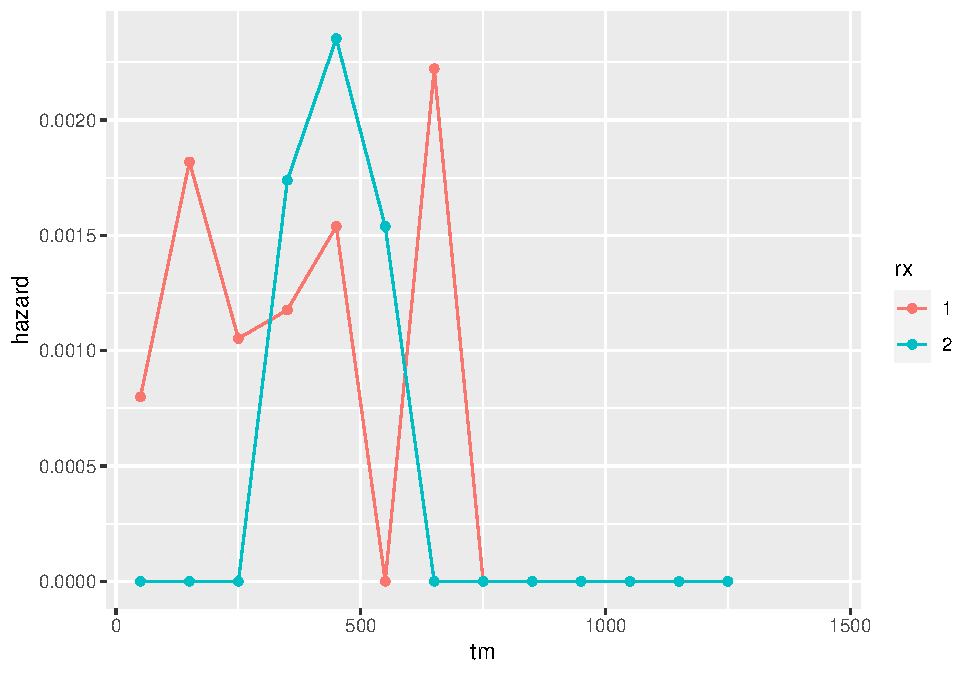
\includegraphics[width=0.8\linewidth]{P8108-hw3-rw2844_files/figure-latex/life_table_hazard-1}

\begin{itemize}
\tightlist
\item
  Plot K-M survival function by \texttt{rx}.
\end{itemize}

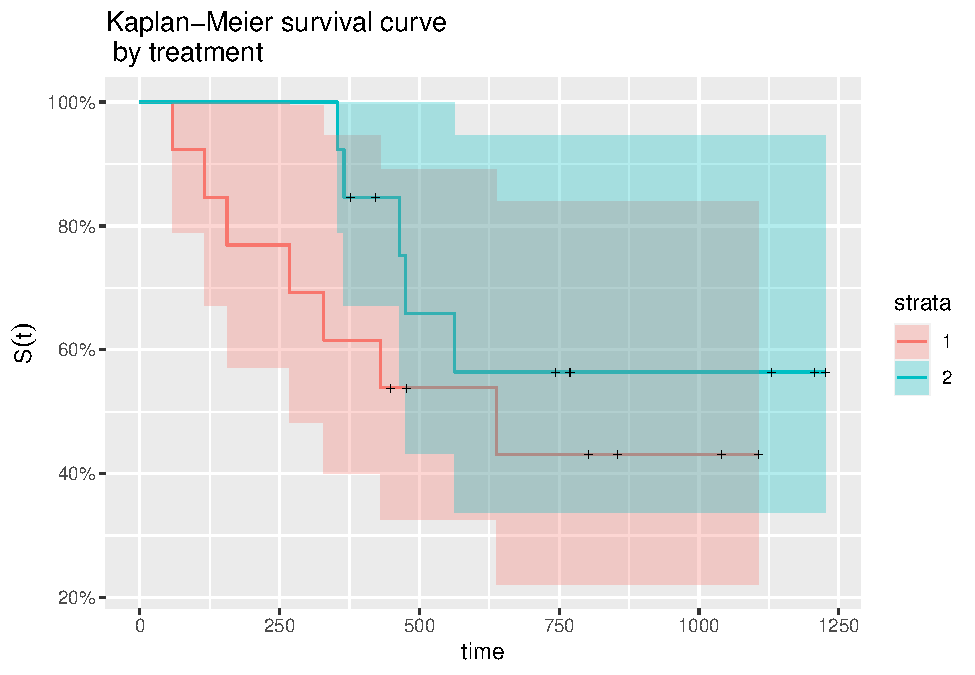
\includegraphics[width=0.8\linewidth]{P8108-hw3-rw2844_files/figure-latex/km_surv_rx-1}
\newpage

\begin{itemize}
\tightlist
\item
  What is the median survival time for each treatment group?
\end{itemize}

\begin{table}[H]

\caption{\label{tab:median_surv}Median survival time by K-M estimation}
\centering
\begin{tabular}[t]{ll}
\toprule
rx & Median Survival (95$\%$ CI)\\
\midrule
1 & 638 (268,--)\\
2 & -- (475,--)\\
\bottomrule
\end{tabular}
\end{table}

\begin{itemize}
\tightlist
\item
  Compare survival function estimations between K-M and F-H methods.
\end{itemize}

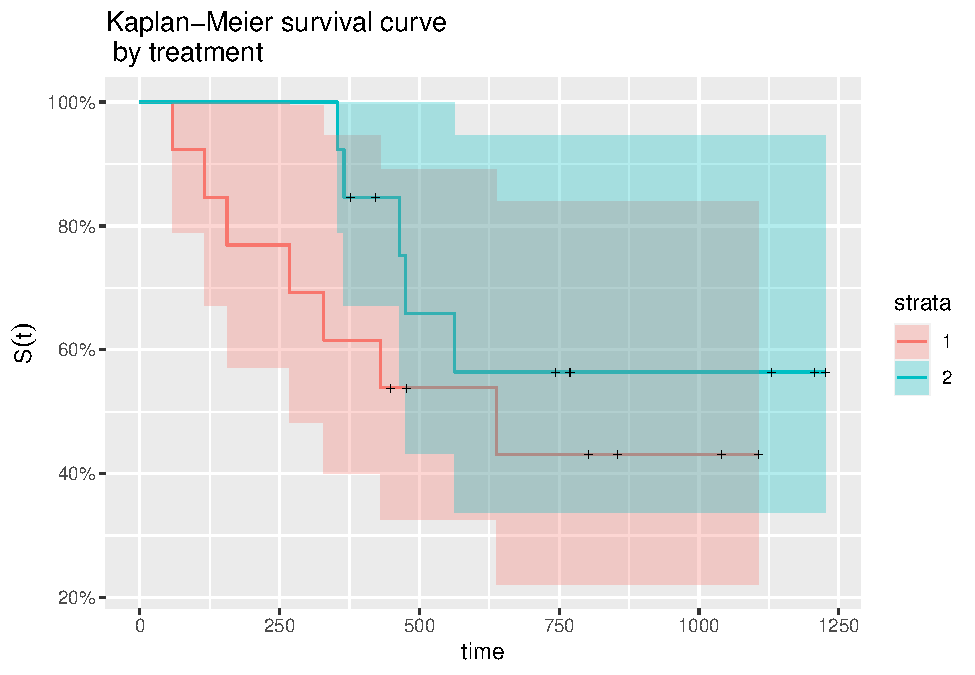
\includegraphics[width=0.6\linewidth]{P8108-hw3-rw2844_files/figure-latex/f_h_survival-1}
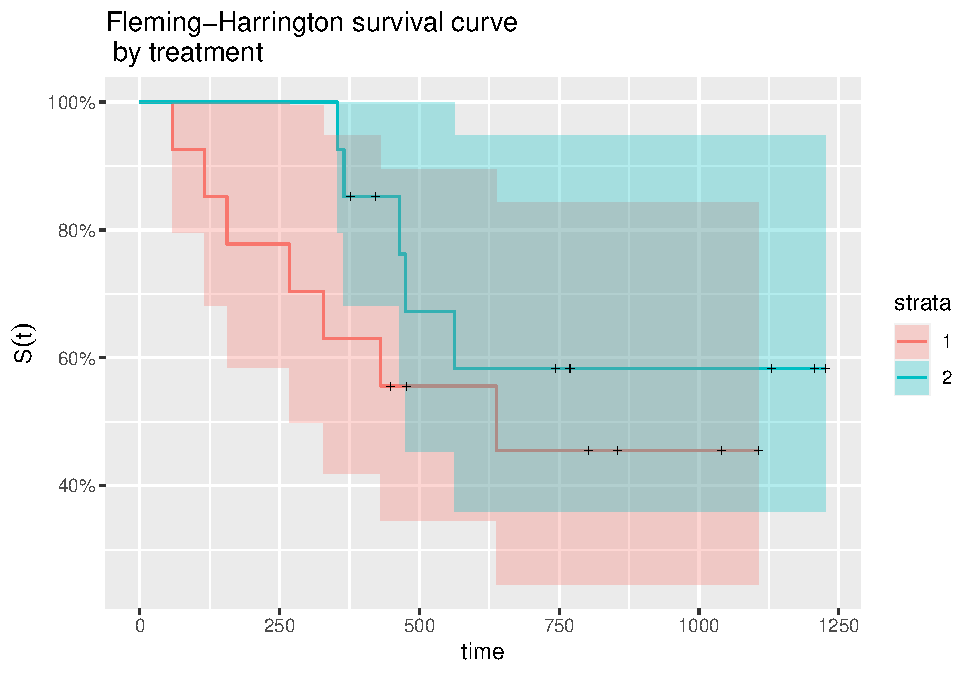
\includegraphics[width=0.6\linewidth]{P8108-hw3-rw2844_files/figure-latex/f_h_survival-2}

\begin{longtable}[t]{rrrrr}
\caption{\label{tab:survival_comp}Survival function estimations between K-M and F-H methods, rx = 1}\\
\toprule
\multicolumn{1}{c}{ } & \multicolumn{2}{c}{K-M estimation} & \multicolumn{2}{c}{F-H estimation} \\
\cmidrule(l{3pt}r{3pt}){2-3} \cmidrule(l{3pt}r{3pt}){4-5}
Time & Survival & Survival Standard Error & Survival & Survival Standard Error\\
\midrule
\endfirsthead
\caption[]{Survival function estimations between K-M and F-H methods, rx = 1 \textit{(continued)}}\\
\toprule
\multicolumn{1}{c}{ } & \multicolumn{2}{c}{K-M estimation} & \multicolumn{2}{c}{F-H estimation} \\
\cmidrule(l{3pt}r{3pt}){2-3} \cmidrule(l{3pt}r{3pt}){4-5}
Time & Survival & Survival Standard Error & Survival & Survival Standard Error\\
\midrule
\endhead

\endfoot
\bottomrule
\endlastfoot
59 & 0.9231 & 0.0801 & 0.9260 & 0.0769\\
115 & 0.8462 & 0.1183 & 0.8519 & 0.1134\\
156 & 0.7692 & 0.1519 & 0.7779 & 0.1453\\
268 & 0.6923 & 0.1849 & 0.7039 & 0.1764\\
329 & 0.6154 & 0.2193 & 0.6298 & 0.2085\\
\addlinespace
431 & 0.5385 & 0.2568 & 0.5558 & 0.2431\\
448 & 0.5385 & 0.2568 & 0.5558 & 0.2431\\
477 & 0.5385 & 0.2568 & 0.5558 & 0.2431\\
638 & 0.4308 & 0.3405 & 0.4551 & 0.3148\\
803 & 0.4308 & 0.3405 & 0.4551 & 0.3148\\
\addlinespace
855 & 0.4308 & 0.3405 & 0.4551 & 0.3148\\
1040 & 0.4308 & 0.3405 & 0.4551 & 0.3148\\
1106 & 0.4308 & 0.3405 & 0.4551 & 0.3148\\*
\end{longtable}

\begin{longtable}[t]{rrrrr}
\caption{\label{tab:survival_comp}Survival function estimations between K-M and F-H methods, rx = 2}\\
\toprule
\multicolumn{1}{c}{ } & \multicolumn{2}{c}{K-M estimation} & \multicolumn{2}{c}{F-H estimation} \\
\cmidrule(l{3pt}r{3pt}){2-3} \cmidrule(l{3pt}r{3pt}){4-5}
Time & Survival & Survival Standard Error & Survival & Survival Standard Error\\
\midrule
\endfirsthead
\caption[]{Survival function estimations between K-M and F-H methods, rx = 2 \textit{(continued)}}\\
\toprule
\multicolumn{1}{c}{ } & \multicolumn{2}{c}{K-M estimation} & \multicolumn{2}{c}{F-H estimation} \\
\cmidrule(l{3pt}r{3pt}){2-3} \cmidrule(l{3pt}r{3pt}){4-5}
Time & Survival & Survival Standard Error & Survival & Survival Standard Error\\
\midrule
\endhead

\endfoot
\bottomrule
\endlastfoot
353 & 0.9231 & 0.0801 & 0.9260 & 0.0769\\
365 & 0.8462 & 0.1183 & 0.8519 & 0.1134\\
377 & 0.8462 & 0.1183 & 0.8519 & 0.1134\\
421 & 0.8462 & 0.1183 & 0.8519 & 0.1134\\
464 & 0.7521 & 0.1670 & 0.7623 & 0.1588\\
\addlinespace
475 & 0.6581 & 0.2139 & 0.6728 & 0.2021\\
563 & 0.5641 & 0.2637 & 0.5832 & 0.2475\\
744 & 0.5641 & 0.2637 & 0.5832 & 0.2475\\
769 & 0.5641 & 0.2637 & 0.5832 & 0.2475\\
770 & 0.5641 & 0.2637 & 0.5832 & 0.2475\\
\addlinespace
1129 & 0.5641 & 0.2637 & 0.5832 & 0.2475\\
1206 & 0.5641 & 0.2637 & 0.5832 & 0.2475\\
1227 & 0.5641 & 0.2637 & 0.5832 & 0.2475\\*
\end{longtable}

\begin{itemize}
\tightlist
\item
  Describe your analyses and write conclusion based on you analyses.
\end{itemize}

\begin{enumerate}
\def\labelenumi{\arabic{enumi}.}
\item
  In both stratums, there are 13 patients. However, there are more
  censored patients in group 2 (\texttt{rx\ =\ 2}) than group 1
  (\texttt{rx\ =\ 1}). The hazard rate of group 1 is higher than group 2
  for most of time.
\item
  According to different survival function estimations, both K-M curves
  and F-H curves show that the survival probability of group 2 is higher
  than group 1.
\item
  The median survival time of group 1 is 638. However, group 2 doesn't
  reach a median survival.
\item
  The estimation by K-M method and F-H method doesn't differ too much.
\end{enumerate}

\hypertarget{reference}{%
\subsection{Reference}\label{reference}}

\begin{enumerate}
\def\labelenumi{\arabic{enumi}.}
\tightlist
\item
  Edmunson, J.H., Fleming, T.R., Decker, D.G., Malkasian, G.D.,
  Jefferies, J.A., Webb, M.J., and Kvols, L.K., Different
  Chemotherapeutic Sensitivities and Host Factors Affecting Prognosis in
  Advanced Ovarian Carcinoma vs.~Minimal Residual Disease. Cancer
  Treatment Reports, 63:241-47, 1979.
\end{enumerate}

\hypertarget{appendix-code-for-this-report}{%
\subsection{Appendix: Code for this
report}\label{appendix-code-for-this-report}}

\begin{Shaded}
\begin{Highlighting}[]
\NormalTok{knitr}\SpecialCharTok{::}\NormalTok{opts\_chunk}\SpecialCharTok{$}\FunctionTok{set}\NormalTok{(}\AttributeTok{echo =} \ConstantTok{FALSE}\NormalTok{, }\AttributeTok{message =} \ConstantTok{FALSE}\NormalTok{, }\AttributeTok{warning =} \ConstantTok{FALSE}\NormalTok{)}
\FunctionTok{library}\NormalTok{(survival)}
\FunctionTok{library}\NormalTok{(tidyverse)}
\FunctionTok{library}\NormalTok{(biostat3)}
\FunctionTok{library}\NormalTok{(ggfortify)}
\FunctionTok{library}\NormalTok{(ggsurvfit)}
\FunctionTok{library}\NormalTok{(gtsummary)}
\FunctionTok{library}\NormalTok{(knitr)}
\FunctionTok{library}\NormalTok{(kableExtra)}
\NormalTok{life\_tab }\OtherTok{\textless{}{-}} \FunctionTok{data.frame}\NormalTok{(}\AttributeTok{Interval =} \FunctionTok{c}\NormalTok{(}\DecValTok{1}\NormalTok{,}\DecValTok{2}\NormalTok{,}\DecValTok{3}\NormalTok{,}\DecValTok{4}\NormalTok{,}\DecValTok{5}\NormalTok{,}\DecValTok{6}\NormalTok{,}\DecValTok{7}\NormalTok{), }
                 \AttributeTok{Period =} \FunctionTok{c}\NormalTok{(}\StringTok{"[0,4)"}\NormalTok{,}\StringTok{"[4,8)"}\NormalTok{,}\StringTok{"[8,12)"}\NormalTok{,}\StringTok{"[12,16)"}\NormalTok{,}\StringTok{"[16,20)"}\NormalTok{,}\StringTok{"[20,24)"}\NormalTok{,}\StringTok{"[24,$}\SpecialCharTok{\textbackslash{}\textbackslash{}}\StringTok{infty$)"}\NormalTok{),}
                 \AttributeTok{d\_i =} \FunctionTok{c}\NormalTok{(}\DecValTok{2}\NormalTok{,}\DecValTok{1}\NormalTok{,}\DecValTok{0}\NormalTok{,}\DecValTok{1}\NormalTok{,}\DecValTok{1}\NormalTok{,}\DecValTok{1}\NormalTok{,}\DecValTok{0}\NormalTok{),}
                 \AttributeTok{c\_i =} \FunctionTok{c}\NormalTok{(}\DecValTok{1}\NormalTok{,}\DecValTok{1}\NormalTok{,}\DecValTok{3}\NormalTok{,}\DecValTok{2}\NormalTok{,}\DecValTok{3}\NormalTok{,}\DecValTok{1}\NormalTok{,}\DecValTok{3}\NormalTok{),}
                 \AttributeTok{n\_i =} \FunctionTok{c}\NormalTok{(}\DecValTok{20}\NormalTok{,}\DecValTok{17}\NormalTok{,}\DecValTok{15}\NormalTok{,}\DecValTok{12}\NormalTok{,}\DecValTok{9}\NormalTok{,}\DecValTok{5}\NormalTok{,}\DecValTok{3}\NormalTok{),}
                 \AttributeTok{n\_i\_prime =} \FunctionTok{c}\NormalTok{(}\FloatTok{19.5}\NormalTok{,}\FloatTok{16.5}\NormalTok{,}\FloatTok{13.5}\NormalTok{,}\DecValTok{11}\NormalTok{,}\FloatTok{7.5}\NormalTok{,}\FloatTok{4.5}\NormalTok{,}\FloatTok{1.5}\NormalTok{),}
                 \AttributeTok{st =} \FunctionTok{c}\NormalTok{(}\FloatTok{1.000}\NormalTok{,}\FloatTok{0.8974}\NormalTok{,}\FloatTok{0.8430}\NormalTok{,}\FloatTok{0.8430}\NormalTok{,}\FloatTok{0.7664}\NormalTok{,}\FloatTok{0.6642}\NormalTok{,}\FloatTok{0.5166}\NormalTok{),}
                 \AttributeTok{ft =} \FunctionTok{c}\NormalTok{(}\FloatTok{0.0257}\NormalTok{,}\FloatTok{0.0136}\NormalTok{,}\DecValTok{0}\NormalTok{,}\FloatTok{0.0192}\NormalTok{,}\FloatTok{0.0256}\NormalTok{,}\FloatTok{0.0369}\NormalTok{,}\ConstantTok{NA}\NormalTok{),}
                 \AttributeTok{ht =} \FunctionTok{c}\NormalTok{(}\FloatTok{0.2703}\NormalTok{,}\FloatTok{0.0156}\NormalTok{,}\DecValTok{0}\NormalTok{,}\FloatTok{0.0238}\NormalTok{,}\FloatTok{0.0357}\NormalTok{,}\FloatTok{0.0625}\NormalTok{,}\ConstantTok{NA}\NormalTok{),}
                 \AttributeTok{se\_st =} \FunctionTok{c}\NormalTok{(}\DecValTok{0}\NormalTok{,}\FloatTok{0.06870}\NormalTok{,}\FloatTok{0.0833}\NormalTok{,}\FloatTok{0.0833}\NormalTok{,}\FloatTok{0.1053}\NormalTok{,}\FloatTok{0.1318}\NormalTok{,}\FloatTok{0.1657}\NormalTok{))}
\FunctionTok{kable}\NormalTok{(life\_tab, }\AttributeTok{col.names =} \FunctionTok{c}\NormalTok{(}\StringTok{"Interval"}\NormalTok{, }\StringTok{"Time Period"}\NormalTok{, }\StringTok{"$d\_i$"}\NormalTok{, }\StringTok{"$c\_i$"}\NormalTok{, }\StringTok{"$n\_i$"}\NormalTok{, }\StringTok{"$n\_i\^{}\{}\SpecialCharTok{\textbackslash{}\textbackslash{}}\StringTok{prime\}$"}\NormalTok{, }\StringTok{"$S(t)$"}\NormalTok{, }\StringTok{"$f(t)$"}\NormalTok{, }\StringTok{"$h(t)$"}\NormalTok{, }\StringTok{"$se(S(t))$"}\NormalTok{), }\AttributeTok{booktabs =}\NormalTok{ T, }\AttributeTok{escape =}\NormalTok{ F, }\AttributeTok{caption =} \StringTok{"Life table estimate"}\NormalTok{) }\SpecialCharTok{\%\textgreater{}\%} \FunctionTok{kable\_styling}\NormalTok{(}\AttributeTok{position =} \StringTok{"center"}\NormalTok{, }\AttributeTok{latex\_options =} \StringTok{"hold\_position"}\NormalTok{) }\SpecialCharTok{\%\textgreater{}\%} \FunctionTok{footnote}\NormalTok{(}\AttributeTok{general =} \StringTok{"Survival functions estimated at the begining of each interval"}\NormalTok{,}\AttributeTok{footnote\_as\_chunk =}\NormalTok{ T)}
\NormalTok{ovarian.rx1 }\OtherTok{\textless{}{-}}\NormalTok{ ovarian[ovarian}\SpecialCharTok{$}\NormalTok{rx }\SpecialCharTok{==} \DecValTok{1}\NormalTok{, ]}
\NormalTok{ovarian.rx2 }\OtherTok{\textless{}{-}}\NormalTok{ ovarian[ovarian}\SpecialCharTok{$}\NormalTok{rx }\SpecialCharTok{==} \DecValTok{2}\NormalTok{, ]}
\NormalTok{ovarian.lt1 }\OtherTok{\textless{}{-}} \FunctionTok{lifetab2}\NormalTok{(}\FunctionTok{Surv}\NormalTok{(futime, fustat)}\SpecialCharTok{\textasciitilde{}}\DecValTok{1}\NormalTok{, }\AttributeTok{data =}\NormalTok{ ovarian.rx1, }\AttributeTok{breaks =}\FunctionTok{seq}\NormalTok{(}\DecValTok{0}\NormalTok{, }\DecValTok{1500}\NormalTok{, }\DecValTok{100}\NormalTok{))}
\NormalTok{ovarian.lt2 }\OtherTok{\textless{}{-}} \FunctionTok{lifetab2}\NormalTok{(}\FunctionTok{Surv}\NormalTok{(futime, fustat)}\SpecialCharTok{\textasciitilde{}}\DecValTok{1}\NormalTok{, }\AttributeTok{data =}\NormalTok{ ovarian.rx2, }\AttributeTok{breaks =}\FunctionTok{seq}\NormalTok{(}\DecValTok{0}\NormalTok{, }\DecValTok{1500}\NormalTok{, }\DecValTok{100}\NormalTok{))}
\NormalTok{ovarian.lt1 }\SpecialCharTok{\%\textgreater{}\%} \FunctionTok{kable}\NormalTok{(}\AttributeTok{booktabs =}\NormalTok{ T, }\AttributeTok{caption =} \StringTok{"Life table, rx=1"}\NormalTok{) }\SpecialCharTok{\%\textgreater{}\%} \FunctionTok{kable\_styling}\NormalTok{(}\AttributeTok{latex\_options =} \FunctionTok{c}\NormalTok{(}\StringTok{"HOLD\_position"}\NormalTok{), }\AttributeTok{font\_size =} \DecValTok{7}\NormalTok{)}
\NormalTok{ovarian.lt2 }\SpecialCharTok{\%\textgreater{}\%} \FunctionTok{kable}\NormalTok{(}\AttributeTok{booktabs =}\NormalTok{ T, }\AttributeTok{caption =} \StringTok{"Life table, rx=2"}\NormalTok{) }\SpecialCharTok{\%\textgreater{}\%} \FunctionTok{kable\_styling}\NormalTok{(}\AttributeTok{latex\_options =} \FunctionTok{c}\NormalTok{(}\StringTok{"HOLD\_position"}\NormalTok{), }\AttributeTok{font\_size =} \DecValTok{7}\NormalTok{)}
\CommentTok{\# hazard: the estimated hazard rate at the midpoint of the intervals.}
\NormalTok{ovarian.lt1}\SpecialCharTok{$}\NormalTok{rx }\OtherTok{=} \FunctionTok{as.factor}\NormalTok{(}\DecValTok{1}\NormalTok{)}
\NormalTok{ovarian.lt2}\SpecialCharTok{$}\NormalTok{rx }\OtherTok{=} \FunctionTok{as.factor}\NormalTok{(}\DecValTok{2}\NormalTok{)}
\NormalTok{ovarian.lt }\OtherTok{\textless{}{-}} \FunctionTok{rbind}\NormalTok{(ovarian.lt1, ovarian.lt2)}
\NormalTok{ovarian.lt}\SpecialCharTok{$}\NormalTok{tm }\OtherTok{\textless{}{-}}\NormalTok{ (ovarian.lt}\SpecialCharTok{$}\NormalTok{tstart }\SpecialCharTok{+}\NormalTok{ ovarian.lt}\SpecialCharTok{$}\NormalTok{tstop)}\SpecialCharTok{/}\DecValTok{2}
\NormalTok{ovarian.lt }\SpecialCharTok{\%\textgreater{}\%} 
  \FunctionTok{ggplot}\NormalTok{(}\AttributeTok{data =}\NormalTok{ ., }\FunctionTok{aes}\NormalTok{(}\AttributeTok{x =}\NormalTok{ tm, }\AttributeTok{y =}\NormalTok{ hazard, }\AttributeTok{group =}\NormalTok{ rx, }\AttributeTok{color =}\NormalTok{ rx)) }\SpecialCharTok{+}
  \FunctionTok{geom\_line}\NormalTok{() }\SpecialCharTok{+} \FunctionTok{geom\_point}\NormalTok{()}
\NormalTok{ovarian.kmfit }\OtherTok{\textless{}{-}} 
\NormalTok{  ovarian }\SpecialCharTok{\%\textgreater{}\%} 
  \FunctionTok{survfit}\NormalTok{(}\FunctionTok{Surv}\NormalTok{(futime,fustat)}\SpecialCharTok{\textasciitilde{}}\NormalTok{rx, }\AttributeTok{data =}\NormalTok{ .)}

\NormalTok{ovarian.kmfit }\SpecialCharTok{\%\textgreater{}\%} \FunctionTok{autoplot}\NormalTok{() }\SpecialCharTok{+}
  \FunctionTok{ylab}\NormalTok{(}\FunctionTok{bquote}\NormalTok{(}\FunctionTok{S}\NormalTok{(t))) }\SpecialCharTok{+}
  \FunctionTok{ggtitle}\NormalTok{(}\StringTok{"Kaplan{-}Meier survival curve }\SpecialCharTok{\textbackslash{}n}\StringTok{ by treatment"}\NormalTok{)}


\CommentTok{\#ovarian.kmfit \%\textgreater{}\% ggsurvfit()}
\NormalTok{km\_median }\OtherTok{=} 
  \FunctionTok{tibble}\NormalTok{(}
    \AttributeTok{rx =} \FunctionTok{as.factor}\NormalTok{(}\FunctionTok{c}\NormalTok{(}\DecValTok{1}\NormalTok{,}\DecValTok{2}\NormalTok{)),}
    \AttributeTok{mediansurvival =} \FunctionTok{c}\NormalTok{(}\StringTok{"638 (268,{-}{-})"}\NormalTok{, }\StringTok{" {-}{-} (475,{-}{-})"}\NormalTok{)}
\NormalTok{  )}
\NormalTok{km\_median }\SpecialCharTok{\%\textgreater{}\%} \FunctionTok{kable}\NormalTok{(}\AttributeTok{booktab =}\NormalTok{ T, }\AttributeTok{escape =}\NormalTok{ F, }\AttributeTok{col.names =} \FunctionTok{c}\NormalTok{(}\StringTok{"rx"}\NormalTok{, }\StringTok{"Median Survival (95$}\SpecialCharTok{\textbackslash{}\textbackslash{}}\StringTok{\%$ CI)"}\NormalTok{), }\AttributeTok{caption =} \StringTok{"Median survival time by K{-}M estimation"}\NormalTok{) }\SpecialCharTok{\%\textgreater{}\%} \FunctionTok{kable\_styling}\NormalTok{(}\AttributeTok{latex\_options =} \FunctionTok{c}\NormalTok{(}\StringTok{"HOLD\_position"}\NormalTok{))}
\NormalTok{ovarian.fhfit }\OtherTok{\textless{}{-}} 
\NormalTok{  ovarian }\SpecialCharTok{\%\textgreater{}\%} 
  \FunctionTok{survfit}\NormalTok{(}\FunctionTok{Surv}\NormalTok{(futime,fustat)}\SpecialCharTok{\textasciitilde{}}\NormalTok{rx, }\AttributeTok{data =}\NormalTok{ ., }\AttributeTok{type =} \StringTok{"fh"}\NormalTok{ )}

\FunctionTok{par}\NormalTok{(}\AttributeTok{mfrow=}\FunctionTok{c}\NormalTok{(}\DecValTok{1}\NormalTok{,}\DecValTok{2}\NormalTok{))}
\NormalTok{ovarian.kmfit }\SpecialCharTok{\%\textgreater{}\%} 
  \FunctionTok{autoplot}\NormalTok{() }\SpecialCharTok{+}
  \FunctionTok{ylab}\NormalTok{(}\FunctionTok{bquote}\NormalTok{(}\FunctionTok{S}\NormalTok{(t))) }\SpecialCharTok{+}
  \FunctionTok{ggtitle}\NormalTok{(}\StringTok{"Kaplan{-}Meier survival curve }\SpecialCharTok{\textbackslash{}n}\StringTok{ by treatment"}\NormalTok{)}
\NormalTok{ovarian.fhfit }\SpecialCharTok{\%\textgreater{}\%} 
  \FunctionTok{autoplot}\NormalTok{() }\SpecialCharTok{+} 
  \FunctionTok{ylab}\NormalTok{(}\FunctionTok{bquote}\NormalTok{(}\FunctionTok{S}\NormalTok{(t))) }\SpecialCharTok{+}
  \FunctionTok{ggtitle}\NormalTok{(}\StringTok{"Fleming{-}Harrington survival curve }\SpecialCharTok{\textbackslash{}n}\StringTok{ by treatment"}\NormalTok{)}
\NormalTok{survival\_tab }\OtherTok{\textless{}{-}} \FunctionTok{tibble}\NormalTok{(}
  \AttributeTok{time =}\NormalTok{ ovarian.fhfit}\SpecialCharTok{$}\NormalTok{time,}
  \AttributeTok{kmsurv =}\NormalTok{ ovarian.kmfit}\SpecialCharTok{$}\NormalTok{surv,}
  \AttributeTok{kmstd =}\NormalTok{ ovarian.kmfit}\SpecialCharTok{$}\NormalTok{std.err,}
  \AttributeTok{fhsurv =}\NormalTok{ ovarian.fhfit}\SpecialCharTok{$}\NormalTok{surv,}
  \AttributeTok{fhstd =}\NormalTok{ ovarian.fhfit}\SpecialCharTok{$}\NormalTok{std.err,}
  \AttributeTok{rx =} \FunctionTok{c}\NormalTok{(}\FunctionTok{rep}\NormalTok{(}\DecValTok{1}\NormalTok{,}\DecValTok{13}\NormalTok{), }\FunctionTok{rep}\NormalTok{(}\DecValTok{2}\NormalTok{,}\DecValTok{13}\NormalTok{))}
\NormalTok{)}
\NormalTok{survival\_tab }\SpecialCharTok{\%\textgreater{}\%} \FunctionTok{filter}\NormalTok{(rx }\SpecialCharTok{==} \DecValTok{1}\NormalTok{) }\SpecialCharTok{\%\textgreater{}\%}\NormalTok{ dplyr}\SpecialCharTok{::}\FunctionTok{select}\NormalTok{(}\SpecialCharTok{{-}}\NormalTok{rx) }\SpecialCharTok{\%\textgreater{}\%} \FunctionTok{kable}\NormalTok{(}\AttributeTok{longtable =}\NormalTok{ T, }\AttributeTok{booktabs =}\NormalTok{ T, }\AttributeTok{caption =} \StringTok{"Survival function estimations between K{-}M and F{-}H methods, rx = 1"}\NormalTok{, }\AttributeTok{col.names =} \FunctionTok{c}\NormalTok{(}\StringTok{"Time"}\NormalTok{, }\StringTok{"Survival"}\NormalTok{, }\StringTok{"Survival Standard Error"}\NormalTok{, }\StringTok{"Survival"}\NormalTok{, }\StringTok{"Survival Standard Error"}\NormalTok{), }\AttributeTok{digits =} \DecValTok{4}\NormalTok{) }\SpecialCharTok{\%\textgreater{}\%} \FunctionTok{add\_header\_above}\NormalTok{(}\FunctionTok{c}\NormalTok{(}\StringTok{" "}\NormalTok{, }\StringTok{"K{-}M estimation"} \OtherTok{=} \DecValTok{2}\NormalTok{, }\StringTok{"F{-}H estimation"} \OtherTok{=} \DecValTok{2}\NormalTok{)) }\SpecialCharTok{\%\textgreater{}\%} \FunctionTok{kable\_styling}\NormalTok{(}\AttributeTok{latex\_options =} \FunctionTok{c}\NormalTok{(}\StringTok{"repeat\_header"}\NormalTok{))}

\NormalTok{survival\_tab }\SpecialCharTok{\%\textgreater{}\%} \FunctionTok{filter}\NormalTok{(rx }\SpecialCharTok{==} \DecValTok{2}\NormalTok{) }\SpecialCharTok{\%\textgreater{}\%}\NormalTok{ dplyr}\SpecialCharTok{::}\FunctionTok{select}\NormalTok{(}\SpecialCharTok{{-}}\NormalTok{rx) }\SpecialCharTok{\%\textgreater{}\%} \FunctionTok{kable}\NormalTok{(}\AttributeTok{longtable =}\NormalTok{ T, }\AttributeTok{booktabs =}\NormalTok{ T, }\AttributeTok{caption =} \StringTok{"Survival function estimations between K{-}M and F{-}H methods, rx = 2"}\NormalTok{, }\AttributeTok{col.names =} \FunctionTok{c}\NormalTok{(}\StringTok{"Time"}\NormalTok{, }\StringTok{"Survival"}\NormalTok{, }\StringTok{"Survival Standard Error"}\NormalTok{, }\StringTok{"Survival"}\NormalTok{, }\StringTok{"Survival Standard Error"}\NormalTok{), }\AttributeTok{digits =} \DecValTok{4}\NormalTok{) }\SpecialCharTok{\%\textgreater{}\%} \FunctionTok{add\_header\_above}\NormalTok{(}\FunctionTok{c}\NormalTok{(}\StringTok{" "}\NormalTok{, }\StringTok{"K{-}M estimation"} \OtherTok{=} \DecValTok{2}\NormalTok{, }\StringTok{"F{-}H estimation"} \OtherTok{=} \DecValTok{2}\NormalTok{)) }\SpecialCharTok{\%\textgreater{}\%} \FunctionTok{kable\_styling}\NormalTok{(}\AttributeTok{latex\_options =} \FunctionTok{c}\NormalTok{(}\StringTok{"repeat\_header"}\NormalTok{))}
\end{Highlighting}
\end{Shaded}


\end{document}
